%!TEX root = ../VorlageBA.tex
\chapter{Grundlagen aus dem IoT für das Thema Smart Home Interior}
\label{cha:grdl}

\addtocontents{toc}{\protect\setcounter{tocdepth}{1}}
\section{Smart Home Aufbau und Funktion}
Ein Smart Home ist ein System, welches automatisch smarte Geräte im Haus steuert. Die smarten Geräte können aber auch zusätzlich durch den Nutzer im Haus gesteuert werden. Dies ist durch verschiedene Kommunikationsmethoden möglich. Diese Kommunikation kann z.B. durch Bluetooth, WiFi oder auch Infrarot durch den Nutzer oder der Smart Home Automatisierung geschehen. Ein smartes Gerät ist ein Gerät, welches mit einem Computer ausgestattet ist und damit die Funktionalität des Gerätes erweitert. Für den Prototypen der Bachelorarbeit wird ein wireless System verwendet. Über das MQTT Protokoll werden die Daten im Netzwerk versendet. Näher erläutert wird dies in Kapitel \ref{cha:arch_pro}. 
\newline
Durch die Automatisierung ist es also möglich, dass bestimmte Interaktionen im Haus nicht mehr manuell vom Bewohner des Hauses getätigt wird. Für jeden Raum wird in der Regel eine unterschiedliche Automatisierung erstellt, da zu unterschiedlichen Zeiten andere smarte Geräte im Raum aktiviert werden. Da im Haus oft Geräte Strom verbrauchen, dabei aber nicht benutzt werden, kann ein Smart Home die smarten Geräte auch so verwalten, dass sie nur dann Strom verbrauchen, wenn sie auch wirklich vom Nutzer aktiv verwendet werden. Sollte das nicht passieren, kann das Smart Home den Stromkreis automatisch unterbrechen. Zusätzlich können damit auch gefährliche Situationen vermieden werden. \citep{sripan2012research}
\newline
Mit den genannten Funktionen ist es möglich verschiedene Smart Home Systeme zu entwickeln. So haben Personen die ohne Hilfe ihren Alltag nicht mehr bewältigen können oder Personen die medizinische Unterstützung brauchen die Möglichkeit, trotzdem selbstständig zu leben. 

\subsection{Neuronale Netze in Smart Homes}
Ein neuronales Netz ist in der Lage das Verhalten von Menschen zu erkennen um so in Smart Homes unter anderem das Strom Management zu verbessern. Anhand von Sensoren wird dann gemessen, unter anderem wie viele Personen sich im Raum befinden und was sie damit wirklich an Strom brauchen. Anhand der Sensorwerte und dem Verhalten der Menschen entscheidet das neuronale Netz dann, welches Gerät ausgeschaltet werden kann. \citep{badlani2011smart} Aus dieser wissenschaftlichen Arbeit ist also zu erkennen, dass ein neuronales Netz durch Interaktionen mit Sensoren die Steuerung der smarten Geräte verwalten kann.

\section{Smart Home Interior}
Das Teilgebiet Smart Home Interior zeigt die digitalisierung der Innenausstattung in einem Smart Home. So wird gezeigt, dass die Möbel im Haus oder der Wohnung als smartes Möbelstück genutzt werden können. Sitzmöbel werden dann als Steuerung anderer smarter Möbel oder Geräte eingesetzt. Außerdem ist es dann möglich für die Möbel eine zusätzliche Automatisierung zu entwickeln und in das Smart Home mit zu integrieren. Smarte Möbel dienen zur passiven Steuerung von smarten Geräten oder Möbelstücken. Der Nutzer muss nicht mehr aktiv ein Tablet oder ähnliches Gerät erst entsperren, die App raussuchen und dann darüber steuern, sondern braucht nur noch eine aktive Interaktion mit den Möbeln haben und diese steuern ohne weiteren Einfluss der Person die Geräte. So spart der Nutzer Zeit und ist nicht mehr gestresst. 
\newline
Für das Sofa ist also nur wichtig, dass sich alle Geräte, welche gesteuert werden sollen in einem Netz befinden. Es werden keine weiteren Apps mehr gebraucht um verschiedene Geräte von verschiedenen Herstellern zu nutzen.

\section{Neuronale Netze zur Klassifizierung}
\label{sec:NNK}
Das folgende Kapitel befasst sich Grundlagen zu neuronalen Netzen. Umfasst wird dabei der Aufbau, wie die Berechnungen auf den Layern stattfinden, wie klassifiziert wird und Allgemeinbegriffe geklärt. Da das Thema zu neuronalen Netzen sehr breit ist, wird hier nur das erläutert, was der Autor auch zur Umsetzung und Evaluation in den späteren Kapiteln benutzt. So sollen später benutzte Fachbegriffe und Methoden nicht in jedem Kapitel neu erklärt werden.

\subsection{Aufbau eines neuronalen Netzes}
Ein neuronales Netz beinhaltet für die Daten der Außenwelt in Form von Zahlenwerten einen Input-Layer. Die Input-Units empfangen diese Werte. Daraufhin werden die Daten weiterverarbeitet und an die Hidden-Units im Hidden-Layer gesendet. Es können mehrere Hidden-Layer je nach Aufgabe des neuronalen Netzes existieren. Nach den Hidden-Layern kommt als letztes der Output-Layer mit den Output-Units. Der Output-Layer gibt die Zahlenwerte aus, die die Vorhersage des neuronalen Netzes als Ergebnisse auch in Form von Zahlenwerten liefern.

\subsection{Berechnung der Inputwerte}
Zwischen den einzelnen Neuronen existieren Gewichtungen  \(w_1 \dots w_n\) welche willkürlich gewählt werden. Diese werden mit den Eingabewerten  \(a_1 \dots a_n\) multipliziert. Diese Multplikationen werden als summiert. Die Aktivierungsfunktion rechnet die Ergebnisse aus dieser Summe aus.
\newline
\[\displaystyle\sum_{i=1}^{n} a_i w_i = (a_1 \cdot w_1 + a_2 \cdot w_2 + \dots + a_{n-1} \cdot w_{n-1} + a_n \cdot w_n)\]
\newline
Zu dem Layer kann dann eine Bias-Unit dazu addiert werden. Dies ist ein konstanter Wert, welcher eins beträgt. So wird die Aktivierungsfunktion später abgeändert, damit sich kein Wert überschneidet.
\newline
Ab der Hidden Schicht wird die Bias-Unit dazu genommen. Da der Input-Layer oft nicht als eigene Schicht in Programmiersprachen betrachtet wird, wird die Bias-Unit auch im neuronalen Netz des Prototypen sofort mit dazu gerechnet.

\subsection{Die Trainingsphase und Testphase mit einlesen von Testdaten}
Bei einem neuronalen Netz gibt es zwei Phasen - die Trainings- und die Testphase. Bei der Trainingsphase werden Testdaten über ein Dataset eingelesen. Dieses Dataset können entweder Vektoren oder Matrizen sein. Anhand dieses Datasets können die Gewichtungen angepasst werden, damit das neuronale Netz, dass trainierte in der Testphase anwenden kann.
\newline
Anders als in der Trainingsphase werden in der Testphase keine neuen Datasets eingelesen. Durch die angepassten Gewichte aus der Trainingsphase kann in der Testphase erkannt werden, was das neuronale Netz gelernt hat. Um zu testen, ob das neuronale Netz eine richtige Vorhersage macht, werden neue Zahlenwerte eingegeben und geprüft.

\subsection{Die sigmoid Aktivitätsfunktion zur Backpropagation}
\label{sec:inp}
Nachdem nun das Dataset eingelesen wurde und die Summe aus der Propagierungsfunktion errechnet ist, wird das Ergebnis in die Aktivitätsfunktion für die Backpropagation eingegeben. Die sigmoid Funktion ist die am häufigsten genutzte Aktivitätsfunktion. Da deren Ergebnisse zwischen null und eins liegen, wird diese Funktion auch für den Prototypen zur Klassifikation benutzt. \citep{Rey2011} Durch das genannte Intervall ensteht ein höheres Spektrum von Möglichkeiten zur Klassifizierung. Anders als bei der step Funktion werden die Ergebnisse größer null mit dem Ergebnis eins ausgegeben. Alle Ergebnisse darunter werden als null ausgegeben.

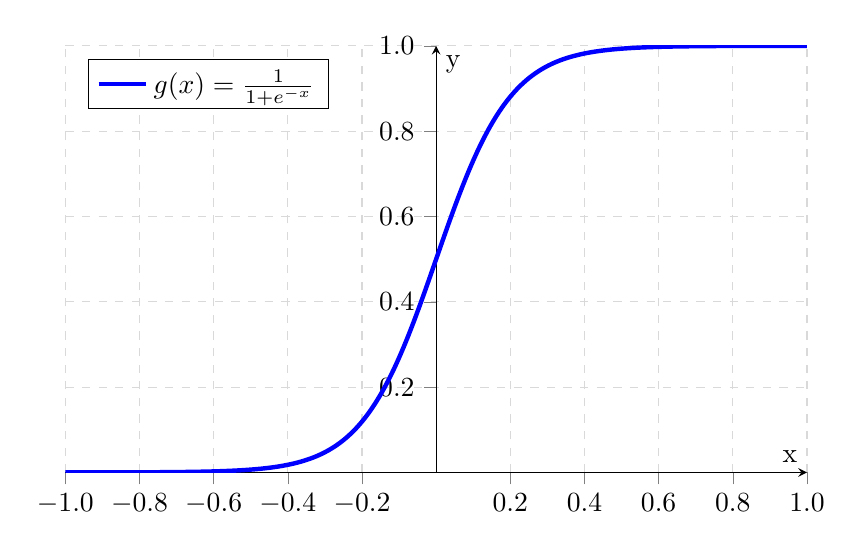
\begin{tikzpicture}
    \begin{axis}[
    	legend pos=north west,
        axis x line=middle,
        axis y line=middle,
        x tick label style={/pgf/number format/fixed,
                            /pgf/number format/fixed zerofill,
                            /pgf/number format/precision=1},
        y tick label style={/pgf/number format/fixed,
                            /pgf/number format/fixed zerofill,
                            /pgf/number format/precision=1},
        grid = major,
        width=11cm,
        height=7cm,
        grid style={dashed, gray!30},
        xmin=-1,     % start the diagram at this x-coordinate
        xmax= 1,    % end   the diagram at this x-coordinate
        ymin= 0,     % start the diagram at this y-coordinate
        ymax= 1,   % end   the diagram at this y-coordinate
        %axis background/.style={fill=white},
        xlabel=x,
        ylabel=y,
        tick align=outside,
        enlargelimits=false]
      % plot the stirling-formula
      \addplot[domain=-1:1, blue, ultra thick,samples=500] {1/(1+exp(-10*x))};
      \addlegendentry{$g(x)=\frac{1}{1+e^{-x}}$}
    \end{axis}
\end{tikzpicture}

\subsection{Backpropagation}
Bei der Backpropagation läuft das neuronale Netz nochmal rückwärts ab um die Gewichte so zu verändern, dass die Fehler auf ein minimum reduziert werden. Wie schon in Kapitel \ref{sec:inp} genannt, wird die sigmoid Funktion verwendet. Wenn aus der sigmoid Funktion die Ergebnisse ausgegeben werden, werden diese an die abgeleitete sigmoid Funktion geschickt. Durch diese abgeleitete Funktion zeigen die Ausgabewerte aus dem feed forward Schritt, wie stark die Gewichtungen abweichen um das gewünschte Ergebnis zu erreichen.
\newline
So wird bei der Backpropagation ein Neuron in zwei Teile aufgeteilt. Auf der rechten Seite ist die Aktivierungsfunktion und auf der linken Seite deren Ableitung. 

\subsection{Ausgabe der Ergebnisse als Klassifizierung}
Das neuronale Netz des Prototypen arbeitet mit der Vorhersage, die Endergebnisse richtig oder falsch zu klassifizieren. In einem zweidimensionalen Diagramm sind die Ergebnisse als x und y Werte im Diagramm dargestellt. Abbildung \ref{fig:nn_class} zeigt ein solches Diagramm mit drei Klassen. Die Punkte stellen die gewünschten Ergebnisse in der richtigen Klasse dar.

\begin{figure}[H]
	\centering
		%[natürliche Breite in Pixeln, natürliche Höhe in Pixeln, Abhängigkeit von der Textbreite]
		\includegraphics[width=0.75\textwidth]{images/nn_classifier.png}
	\caption{Beispiel eines classifiers}
	\label{fig:nn_class}
\end{figure}

Um die Ergebnisse richtig zu klassifzieren, müssen die korrekten Klassifizierungen in die Richtung des Wertes eins gehen und alle anderen Ergebnisse Richtung null. Daher ist wieder zu erwähnen, dass die sigmoid Funktion für dieses neuronale Netz geeignet ist.

\section{MQTT zur Datenübertragung}
MQTT ist ein Protokoll, welches mit der Publish/Subscribe Methode arbeitet. Mikrocontroller und Sensoren publishen ihre Daten an den MQTT Broker. Der Broker speichert diese Daten bis Subscriber diese Nachrichten zugesendet bekommen. Jeder Subscriber bekommt diese Nachrichten dann gleichzeitig. Diese Clients können ihre Daten wiederum auch publishen und wieder an neue Geräte die Subscriber sind versenden. Als Clients sind intelligente Geräte gemeint wie Mikrocontroller oder PCs. Publisher versenden also Nachrichten und Subscriber erhalten diese. Also kann ein Client sowohl Publisher als auch Subscriber sein. \citep{soni2017survey} Für die Kommunikation ist demnach ein TCP-Stack und das MQTT-Protokoll vorausgesetzt. Zusätzlich ist eine Verbindung zum MQTT-Broker erforderlich wo der Typ des Netzes aber unwichtig ist. Die Anzahl der Clients die aktiv als Subscriber oder Publisher dienen ist nicht relevant. Wichtig ist dabei nur, dass der Broker funktioniert und Verfügbar für die Clients ist. Außerdem ist zu erwähnen, dass es nicht relevant ist, dass sowohl Publisher als auch Subscriber gleichzeitig aktiv sein müssen. Der Broker kann die Nachrichten auch dann noch übermitteln, auch wenn der Publisher nicht mehr aktiv ist. Damit Nachrichten versendet werden, gibt es die topics. Dabei ist es nicht wichtig, über welche Struktur die Nachricht aufgebaut ist. \citep{Trojan2017}
\newline
MQTT ist mit dieser Methode also ein Protokoll, was passend für diesen Prototypen ist, da es für das Senden von Sensordaten in einem Wireless Network ausgelegt ist. Der Mosquitto Broker findet in diesem System Verwendung zur Nachrichtenübermittlung. 
\newline
\newline
Das Protokoll hat drei Stufen des Quality of Service. Diese werden in der Tabelle \ref{tab:tableqos} dargestellt. Die Stufen dienen zur Sicherung der Nachrichtenübermittlung auch wenn das Netz Störungen beim übertragen hat.

\begin{table}[ht]
	\centering
	\caption[Tabellarische Darstellung der QoS Level]{Tabellarische Darstellung der QoS Level \citep{soni2017survey}}
		\vspace{1.0em}	
	\begin{tabular}{| l | l | p{5cm}|}
		\hline
		\rowcolor[gray]{0.9}\textbf{Stufen} & \textbf{Häufigkeit} & \textbf{Beschreibung} \\
		\hline
		\hline
		0 & höchstens eine Nachricht & Es wird maximal eine Nachricht versendet, ohne eine Garantie, dass diese auch ankommt \\
		\hline
		1 & mindestens eine Nachricht & Es ist möglich, dass eine Nachricht mehr als einmal versendet wird\\
		\hline
		2 & genau eine Nachricht & Eine Nachricht wird mit einem Four-Way Handshake versendet\\
		\hline
	\end{tabular}
	\label{tab:tableqos}
\end{table}

\section{Sensoren für die Interaktionen auf dem Sofa}
\subsection{Erläuterung des Raspberry Pi 3 und des ESP32}
Der Raspberry Pi 3 ist ein Einplatinen Computer, auf dem das Betriebssystem Raspbian installiert ist. Das Betriebssystem basiert auf Linux Debian und läuft in der aktuellen Version 10 - Buster. Neben den Möglichkeiten den Raspberry Pi für einfachere Anwendungen zu Verwenden ist es auch möglich, verschiedene Sensoren an dessen GPIO Pins anzuschließen. Der Raspberry Pi 3 hat einen eine interne WiFi Karte und kann damit in einem WLAN Netzwerk eingebunden werden. Dies wird gebraucht, da der Prototyp in einem lokalen Netzwerk ausgeführt wird.
\newline
Der ESP32 ist ein Mikrocontroller, welcher als Nachfolger vom ESP8266 weitere GPIO Pins bekommen hat um mehr als einen Analogen Sensor anschließen zu können. Ein ESP32 hat ein Live Betriebssystem und kann nur ein Programm ausführen, welches vorher hochgeladen werden muss. 

\subsection{Sensoren die für den Prototypen verwendet werden}
Für den aktuellen Prototyp werden Ultrasonic Sensoren und Force Sensitive Resistors verwendet. 
Diese reichen aus um Sitz- und Liegepositionen der Nutzer zu erkennen. Der Ultrasonic Sensor misst anhand von Wellen den Abstand zwischen dem Sensor und einem Gegenstand.
\newline
Der FSR misst anhand des elektrischen Widerstands den Druck, welcher zwischen 100 Gramm und 10 Kilogramm beträgt. Bei allen Gewichten über zehn Kg zeigt der Sensor immer den höchsten Wert. \citep{florez2010calibration}
Sie sind aus zwei Polymer Schichten gebaut. Eine leitende Oberfläche und eine andere an die erste bindende Schicht mit Elektroden. \citep{hollinger2006evaluation} Diese Sensoren werden also dafür verwendet um zu erkennen, wann die Personen Druck auf sie einüben indem sie ihn mit ihrem Gewicht auslösen. Als FSRs werden die interlink FSR Sensoren eingesetzt.

\section{Prototyp aus dem Praxisprojekt}
Im Rahmen des Praxisprojekts entsteht ein Prototyp, welcher die Interaktionen als Regelsystem mit sieben Regeln verwaltet. Ein ESP32 misst die Sensordaten von zwei FSRs und einem Ultrasonic Sensor. Jeder Sensor wird als MQTT Client deklariert und sendet Codes die er aus den Sensordaten erstellt. Zusätzlich messen zwei ESP8266 die Daten von Flex Sensoren, welche den Widerstand durch ihre Biegung messen. Dies erwies sich aber als ein Nachteil, da die Biegung erst ab 45 Grad gemessen wird. Ein Raspberry Pi 2 führt einen MQTT Broker Service aus und kann Daten von den ESPs empfangen, die über die Publish Methode die Codes versenden. Auf dem Raspberry Pi 2 läuft zusätzlich ein Python Programm, welches die Codes als Subscriber empfängt und im Regelsystem verwaltet. Die Regeln werden als Codes neu an den MQTT Broker gepublished und können dann von jedem beliebigen Subscriber empfangen werden. \citep{Schroeder2019} 
\newline
Was bei der Nutzung des Regelsystems aber nicht beachtet wurde, sind die Ausreißer der FSR Sensorwerte. Mit dem Regelsystem zielt man darauf ab, dass die FSRs immer bei nicht benutzung den Wert null haben und wenn sie besetzt sind, den Wert 1024. Während des Tests sind diese Ausreißer immer wieder aufgefallen. Damit passiert es also, dass manchmal der FSR Sensor eine Interaktion erkennt, obwohl keine stattfindet.
Kapitel \ref{sec:ums_nn} zeigt die Lösung im neuronalen Netz und Kapitel \ref{sec:arch_sofa} stellt die Hardware Lösung im Prototypen dafür dar.